\chapter{Optical Cavities}

Consider a simple Fabry-Perot resonator consisting of three mirrors, of which only one is responsible for coupling light in and out of the resonator, as in Figure \ref{fig:fabry.perot}. The field can be written as a function of the position along the internal cavity path, ranging form $0$ to $L$. Our goal is to study the interaction between these fields, and how they relate to the properties of the resonator.

\begin{figure}[H]
    \centering
    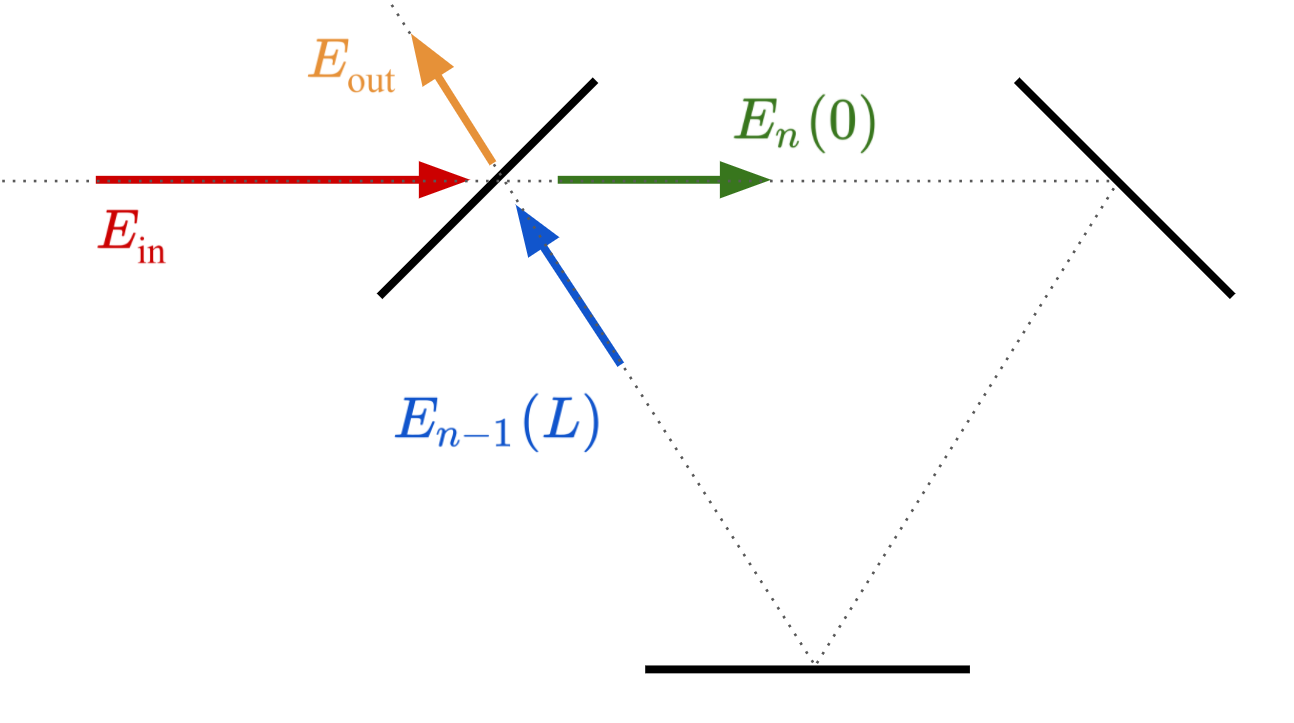
\includegraphics[width=0.75\linewidth]{Figuras/fabry-perot model.png}
    \caption{Fabry-perot resonator.}
    \label{fig:fabry.perot}
\end{figure}

This result will be demonstrated in such a  way as to make it easily generalizable to more complex systems. In that sense, the inside of the cavity can be treated as a ``black box'' containing only one port where the light can couple in and out, and inside of which the field gains some phase and undergoes some loss (with few adjustments it can also exhibit nonlinear effects).

We begin by writing a simple beam-splitter equation for the fields described in Figure \ref{fig:fabry.perot}, that is
%
\begin{equation}
    \begin{cases}
    E_{out}=\sqrt{T}E_{n-1}(L)-\sqrt{R}E_{in}\\[0.5cm]
    E_{n}(0)=\sqrt{R}E_{n-1}(L)+\sqrt{T}E_{in}
    \end{cases}
    \label{eq:beam splitter}
\end{equation}
%
and the goal is to write the change in the electric field between two consecutive round-trips
%
\begin{equation}
    \Delta E = E_n(0)-E_{n-1}(0)
\end{equation}
for each trip, we assume the field must undergo a phase shift proportional to its propagation constant $\beta(\omega)$. Additionally, losses can be modeled as an exponential decay along the length $L$ of the cavity, determined by an ``attenuation coefficient'' $\alpha$. Finally, losses due to imperfect reflection by the intra-cavity mirrors can be summarized by a reflection coefficient $\sqrt{R_b}$ (distinct from the coefficient $\sqrt{R}$ at the coupling mirror), then
%
\begin{equation}
    E_{n-1}(L)=\exp{i\beta(\omega)L}\exp{-\frac{\alpha}{2}L}\sqrt{R_b}E_{n-1}(0)
\end{equation}
Notice that the $1/2$ factor in the exponent of the attenuation term is convenient when we switch to a description in terms of energy rather than amplitude, since the former is proportional to the square of the latter. The function $\beta(\omega)$ in the phase shift term can be expanded as a Taylor series around the resonance frequency $\omega_0$ and the detuning $\delta\omega=\omega-\omega_0$, such that
\begin{equation}
    \exp{i\beta(\omega)L}=\exp(i\beta(\omega_0)L)\exp(i\beta^{(1)}\delta\omega L)\dots
\end{equation}
%
where I have only kept terms up to first order in $\delta\omega$. The first term is equal to one by the definition of the \textit{resonance} frequency. The resonance frequency of a Fabry-Perot cavity is precisely one in which the field will accumulate a $\phi=2\pi$ phase-shift at each round trip, thus $\beta(\omega_0)L=2\pi$. We are now left with
%
\begin{equation}
    E_{n-1}(L)=\exp(i\beta^{(1)}\delta\omega L)\exp(-\frac{\alpha}{2}L)\sqrt{R_b}E_{n-1}(0).
\end{equation}
Ignoring higher order terms in $i\delta\omega L$ (near-resonance operation), $\alpha L$ (low attenuation) and $T_b$ (high reflectance of the intra-cavity mirrors), the expression becomes
\begin{equation}
    E_{n-1}(L)=(1+i\beta^{(1)}\delta\omega L)\left(1-\frac{\alpha L}{2}\right)\left(1-\frac{T_b}{2}\right)E_{n-1}(0)
\end{equation}
where we have used the general relation $\sqrt{R}=\sqrt{1-T}$. Carrying out the multiplication we get to
\begin{equation*}
    E_{n-1}(L)=\left(1-\frac{\alpha L}{2}+i\beta^{(1)}\delta\omega L - \frac{1}{2}i\beta^{(1)}\delta\omega L^2\alpha\right)\left(1-\frac{T_b}{2}\right)E_{n-1}(0),
\end{equation*}
discarding the last term in the first parenthesis
\begin{equation*}
    E_{n-1}(L)=\left(1-\frac{\alpha L}{2}+i\beta^{(1)}\delta\omega L\right)\left(1-\frac{T_b}{2}\right)E_{n-1}(0),
\end{equation*}
\begin{equation*}
    E_{n-1}(L)=\left(1-\frac{T_b}{2}-\frac{\alpha L}{2}+\frac{1}{4}\alpha L T_b+i\beta^{(1)}\delta\omega L-i\beta^{(1)}\delta\omega L\frac{T_b}{2}\right)E_{n-1}(0)
\end{equation*}
Finally, ignoring the other second-order terms,
\begin{equation}
    E_{n-1}(L)=\left(1+i\beta^{(1)}\delta\omega L - \frac{1}{2}(T_b+\alpha L)\right)E_{n-1}(0).
\end{equation}
Now, going back to the beam-splitter equation above,
\begin{equation}
    \begin{aligned}
        E_n(0)&=\sqrt{R}E_{n-1}(L)+\sqrt{T}E_{in}\\
        &=\left(1-\frac{T}{2}\right)\left(1+i\beta^{(1)}\delta\omega L - \frac{1}{2}(T_b+\alpha L)\right)E_{n-1}(0)+\sqrt{T}E_{in}\\
        &\approx\left(1+i\beta^{(1)}\delta\omega L - \frac{1}{2}(T+T_b+\alpha L)\right)E_{n-1}(0)+\sqrt{T}E_{in}
    \end{aligned}    
\end{equation}
we get to a position where we can finally write the change in the electric field between two consecutive round-trips
\begin{equation}
    \begin{aligned}
        \Delta E&=E_n(0)-E_{n-1}(0)\\
        &=\left(1+i\beta^{(1)}\delta\omega L - \frac{1}{2}(T+T_b+\alpha L)\right)E_{n-1}(0)+\sqrt{T}E_{in}-E_{n-1}(0)\\
        &=\left(i\beta^{(1)}\delta\omega L - \frac{1}{2}(T+T_b+\alpha L)\right)E_{n-1}(0)+\sqrt{T}E_{in}\\
        &\equiv \left(i\beta^{(1)}\delta L-\frac{\gamma}{2}\right)E_{n-1}(0)+\sqrt{T}E_{in}
    \end{aligned}    
\end{equation}
where I have defined $\gamma=(T+T_b+\alpha L)/2$ and $\delta\omega=\delta$ for simplicity. If we divide the whole equation by $t_R=L/v_g=L\beta^{(1)}$, we get to
\begin{equation}
    \frac{\Delta E}{t_R}=\left(i\delta-\frac{\gamma}{2t_R}\right)E_{n-1}(0)+\frac{\sqrt{T}}{\sqrt{t_R}}\frac{E_{in}}{\sqrt{t_R}}.
\end{equation}
Notice now that the energy density inside the cavity is such that
\begin{equation}
    U\propto |E|^2\;\;\;\Rightarrow\;\;\;U=c|E|^2=\hbar\omega\Bar{n}\equiv\hbar\omega|\alpha|^2,
\end{equation}
which allows us to write a correspondence between the field $E$ and the dimensionless quantity $\alpha$ related to the average number of photons
\begin{equation}
    E=\frac{\hbar\omega}{C}\alpha=\frac{1}{K}\alpha.
\end{equation}
So in order for the whole equation to be in terms of $E$, we should multiply it all by the constant $K$
\begin{equation}
    K\frac{\Delta E}{t_R}=\left(i\delta-\frac{\gamma}{2t_R}\right)KE_{n-1}(0)+\frac{\sqrt{T}}{\sqrt{t_R}}K\frac{E_{in}}{\sqrt{t_R}}.
\end{equation}
Finally, we take the limit where the number of round-trips is infinite, such that $t_R\rightarrow 0$ and all the field terms become alpha terms. Once we make
\begin{equation}
    \sqrt{\gamma_{in}}=\frac{\sqrt{T}}{\sqrt{t_R}}\;\;\;\text{and}\;\;\;\alpha_{in}=\lim_{n\rightarrow\infty}\left(K\frac{E_{in}}{t_R}\right)\;\;\text{such that}\;\;|\alpha_{in}|^2=\frac{\Bar{n}}{t_R}
\end{equation}
Thus, the final expression for the Fabry Perot equation is
\begin{equation}
    \boxed{\frac{d\alpha}{dt}=\left(i\delta-\frac{\gamma}{2}\right)\alpha+\sqrt{\gamma_{in}}\alpha_{in}}
    \label{eq:final.fabry.perot}
\end{equation}

\section*{Properties}
Consider the case where the resonator is operating in a steady state, such that the derivative in Equation \ref{eq:final.fabry.perot} is zero
\begin{equation}
    \frac{d\alpha}{dt}=0\;\;\;\Rightarrow \alpha=\frac{\sqrt{\gamma_{in}}\alpha_{in}}{\left(\frac{\gamma}{2}-i\delta\right)}
\end{equation}
We should hold on to that result for a second, and take a look at what can be said about the cavity's emission. Equation \ref{eq:beam splitter} told us that


